\subsection{Session: Deep Learning}

This section appeared to be quite diverse on topics and it was hard to understand the flow. However, there still were a couple of talks that I found to be interesting.

\spacerule
\subsubsection{Spotlight: What if Neural Networks had SVDs? \cite{mathiasen2020neural}}

Talk by \textit{Alexander Mathiasen} \\

{\bf Motivation:} the SVD allows faster computation of some matrix operations commonly used by Neural Networks: 
\begin{itemize}
  \item Spectral Normalization \cite{MiyatoKKY18} - a very popular technique to stabilize training of Generative Adversarial Networks (GANs)
  \item matrix inverse and Cayley transform - essential to train flow-based models (type of generative models, alternatives to GANs) \cite{kingma2018glow}
  \item other applications such as matrix determinant and matrix exponential are less practical
  \item 
\end{itemize} \\

{\bf Observation:} computation of SVD can be included in the computation of gradient descent. 
In this case, getting SVD results from a layer will take no time (because values are already computed when a user asks for them). \\

{\bf Problem:} SVD cannot be directly directly formulated as a part of gradient descent step: 
\begin{equation} 
  \hat{M} != M - \eta\nabla_{M}
\end{equation} 

{\bf Method:} develop the Fast Householder Multiplication (FastH) method, which is a modification of the Householder transformation that supports parallel execution to better utilize GPU resources and includes some linear algebra tricks \\

{\bf Conclusions:} new method is fast on small matrices and also his complexity grows very slowly with grows of size of the decomposed matrix: \\
\begin{center}
  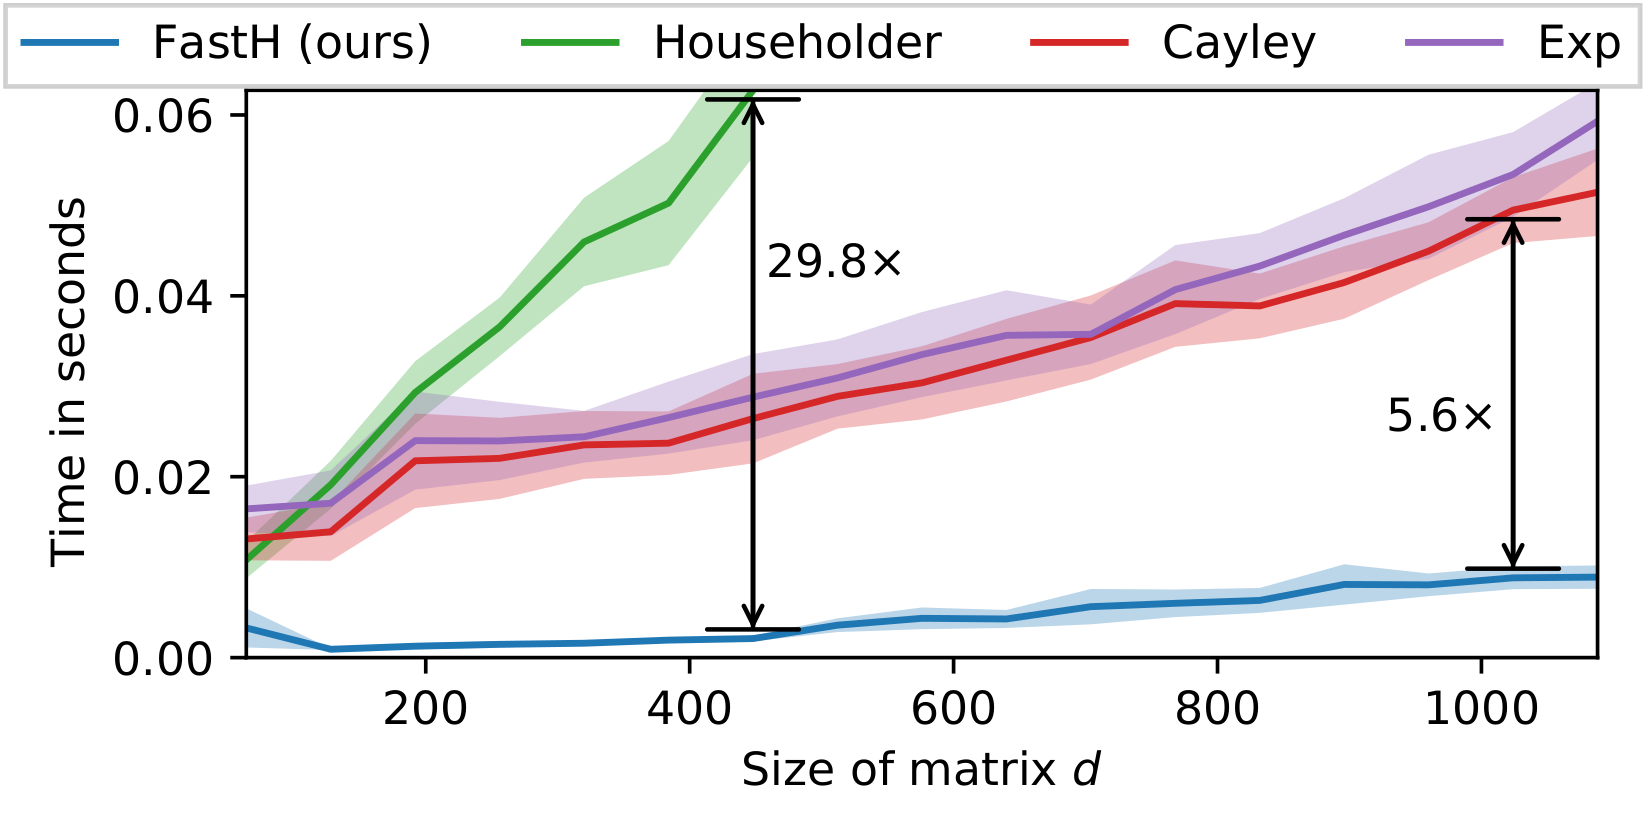
\includegraphics[scale=0.2]{neurips-2020/images/fastH.png} \\
\end{center}

{\bf Key takeaway:} \href{https://github.com/AlexanderMath/fasth/}{code in released on GitHub}, try it out. \\


\subsubsection{Spotlight: Triple descent and the two kinds of overfitting: where & why do they appear? \cite{dascoli2020triple}}

Talk by \textit{Stéphane d'Ascoli} \\

{\bf Motivation:} when we increase the number of parameters in a machine learning model we expect loss function to decrease and then increase following the U-shape curve following the systematic bias-variance trade-off. When we increase the dataset size we expect train loss value to diminish and generalization to improve.
However, this not something that happens in real Deep Learning. \\

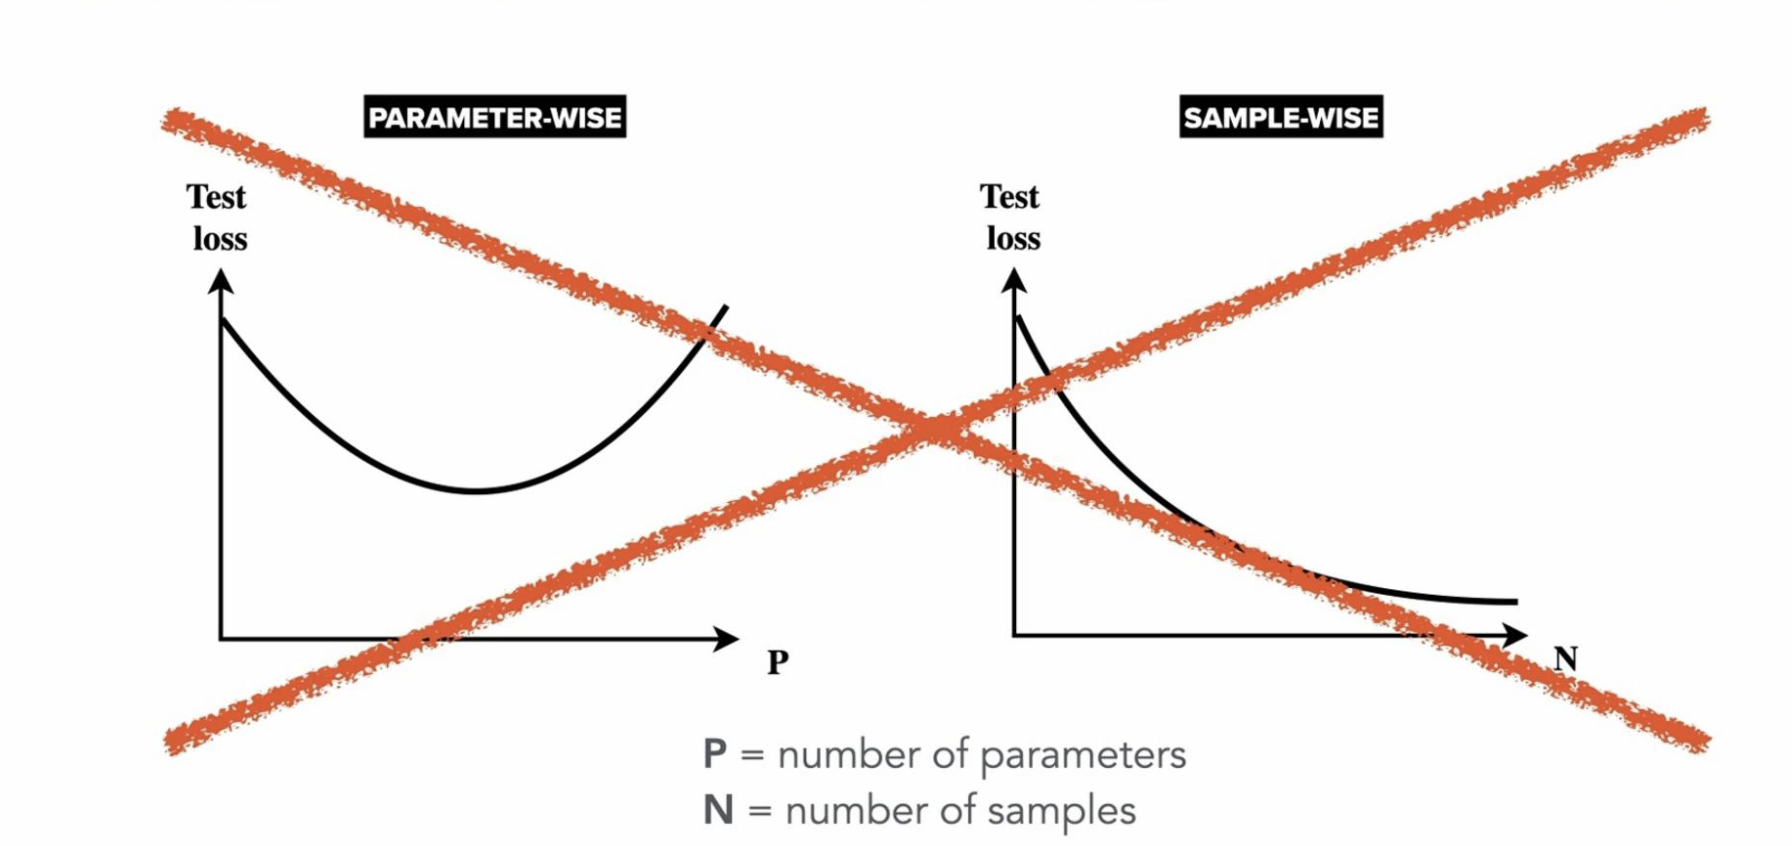
\includegraphics[scale=0.25]{neurips-2020/images/Screenshot 2020-12-09 at 18.45.09.png}
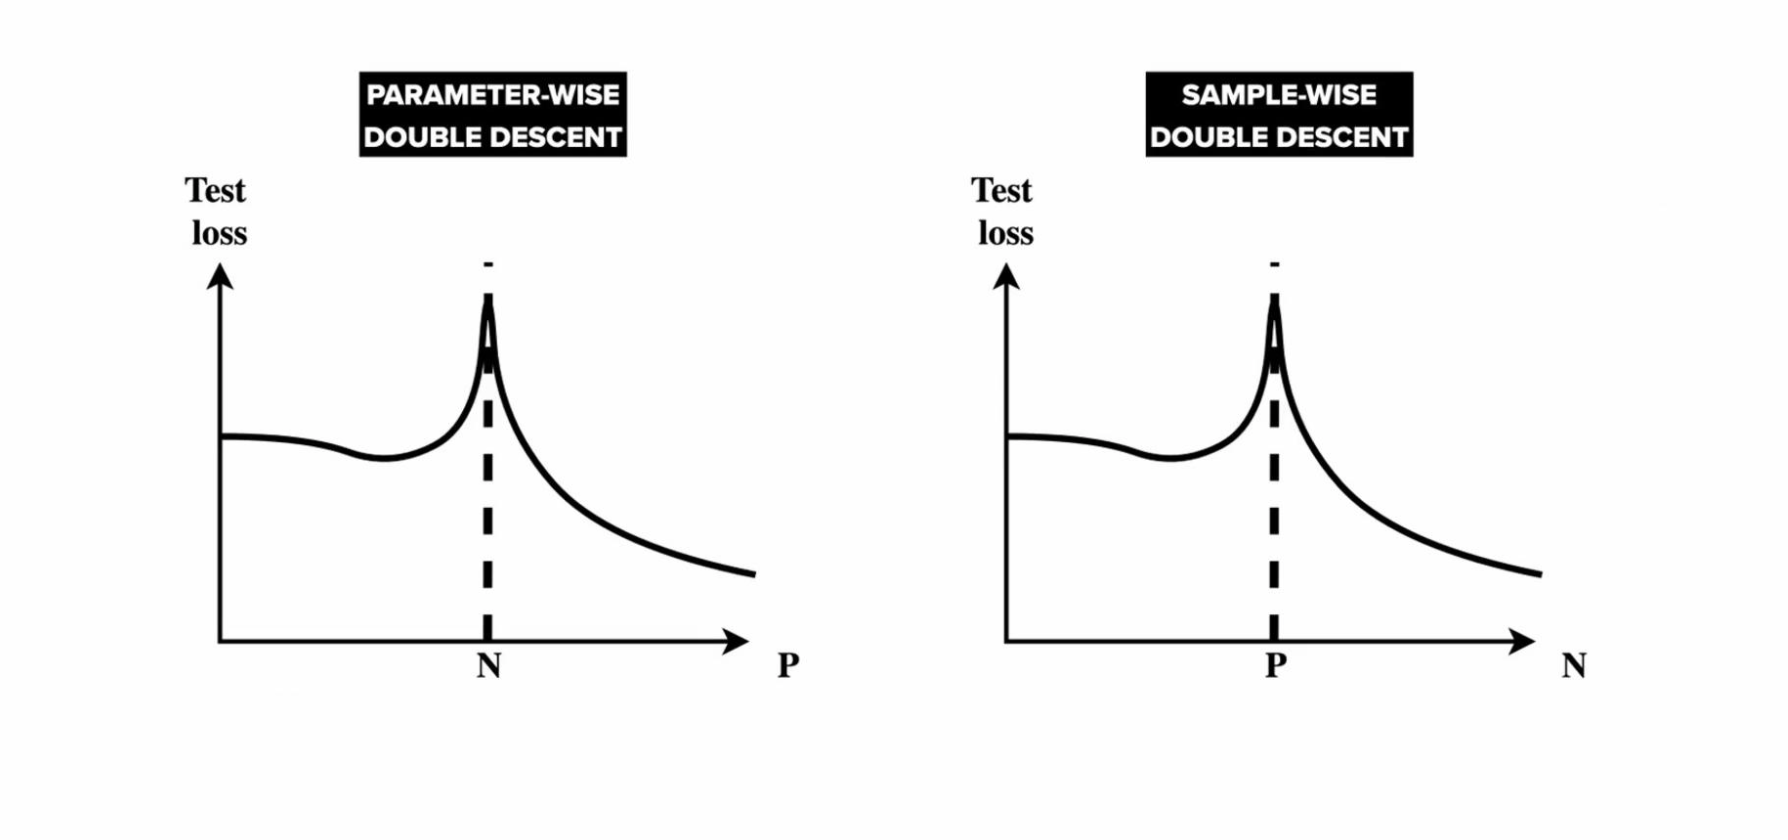
\includegraphics[scale=0.25]{neurips-2020/images/Screenshot 2020-12-09 at 18.48.59.png} \\

In this work authors focus on the sample-wise double descent curve. It was discovered in 2018 by Belkin et. al. \cite{belkin2019reconciling} and the over-fitting peak happen to co-inside with the interpolation threshold whether training loss becomes non-zero. Much earlier similar phenomena was discovered for linear models (perception) [LeCun et. al., 1991]. \\

{\bf Observation:} the non-linear peak occurs when number of training parameters $P$ is of the same order as the number of training examples $N$. However, in linear model the over-fitting peak occurs when $N$ is of the same order as input dimension $d$. Morevoer, in case of noisy regression task with weakly non-linear activation functions both peaks can be observed simultaneously. \\ 
\begin{center}
  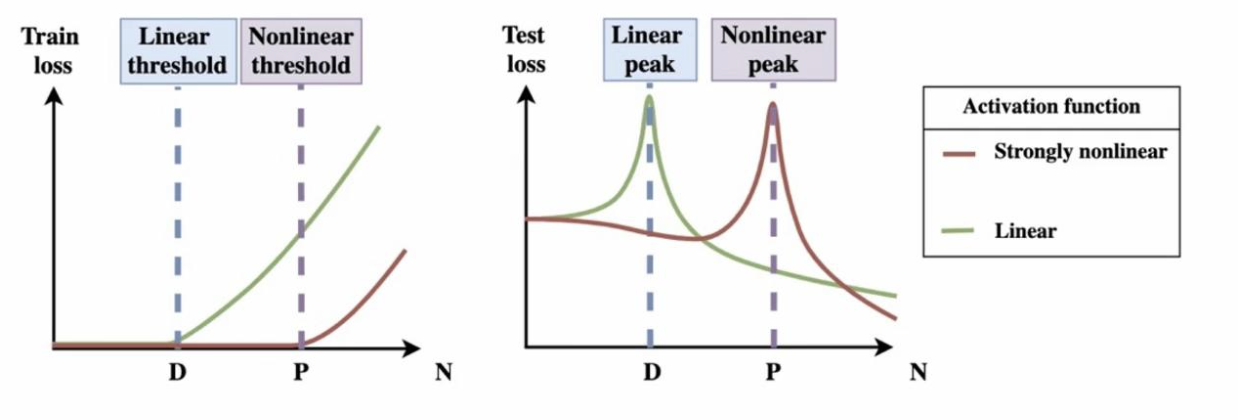
\includegraphics[scale=0.5]{neurips-2020/images/Screenshot 2020-12-09 at 19.14.11.png} \\
\end{center}

{\bf Goal of the work:} understand what cause these peaks. \\

{\bf Method:} vary degree on non-linearity of activation functions, analyse eigenvalues of Gramm matrices of tested models (fully connected).

{\bf Conclusions:} 
\begin{itemize}
  \item Linear peak is caused by the variance due to the noise in the labels
  \item Non-linear peak occurs due to initialization of random features
\end{itemize}
The consequence of this is that even if there is no noise in labels, non-linear peak when $N$ equal to $P$ still occurs, whereas the linear peak vanishes. \\

{\bf Key takeaway:} this explains why in Deep Learning we experience over-fitting even there is no noise in the dataset. \\



\subsection{Session: Social/Adversarial Learning}
\subsubsection{Spotlight: Guided Adversarial Attack for Evaluating and Enhancing Adversarial Defenses \cite{SriramananABR20}}

Talk by \textit{Gaurang Sriramanan} \\

{\bf Motivation:} current SOTA PGD attack may not be effective due to the non-convex nature of many Machine learning tasks leading to correct response from the model under attack. Existing modifications such as performing PGD attack sequentionally with respect to several targets introduces additional computational cost. \\

{\bf Observation:} better selection of initial gradient direction leads to a stronger attack. \\

{\bf Method:} introduce the new attack called Guided Adversarial Margin Attack (GAMA):

\begin{equation}
    L = -f^{y}_{\theta}(\tilde{x}) + \max_{j \neq y} f^{j}_{\theta}(\tilde{x}) + \lambda \cdot ||f_{\theta}(\tilde{x}) - f_{\theta}(x))||^2_2 
    \label{eq:gama}
\end{equation}

First two terms of equation \ref{eq:gama} correspond to the maximum margin loss in probability space. Next, there is a smoothing term, which is represented as L2 distance between probability vectors of clean image and the perturbed image. \\

{\bf Observation:} introduction of a relaxation term (regularization) leads to smoother loss function (more convex problem) and hence better outcome of the attack. \\

\begin{figure}
  \centering
  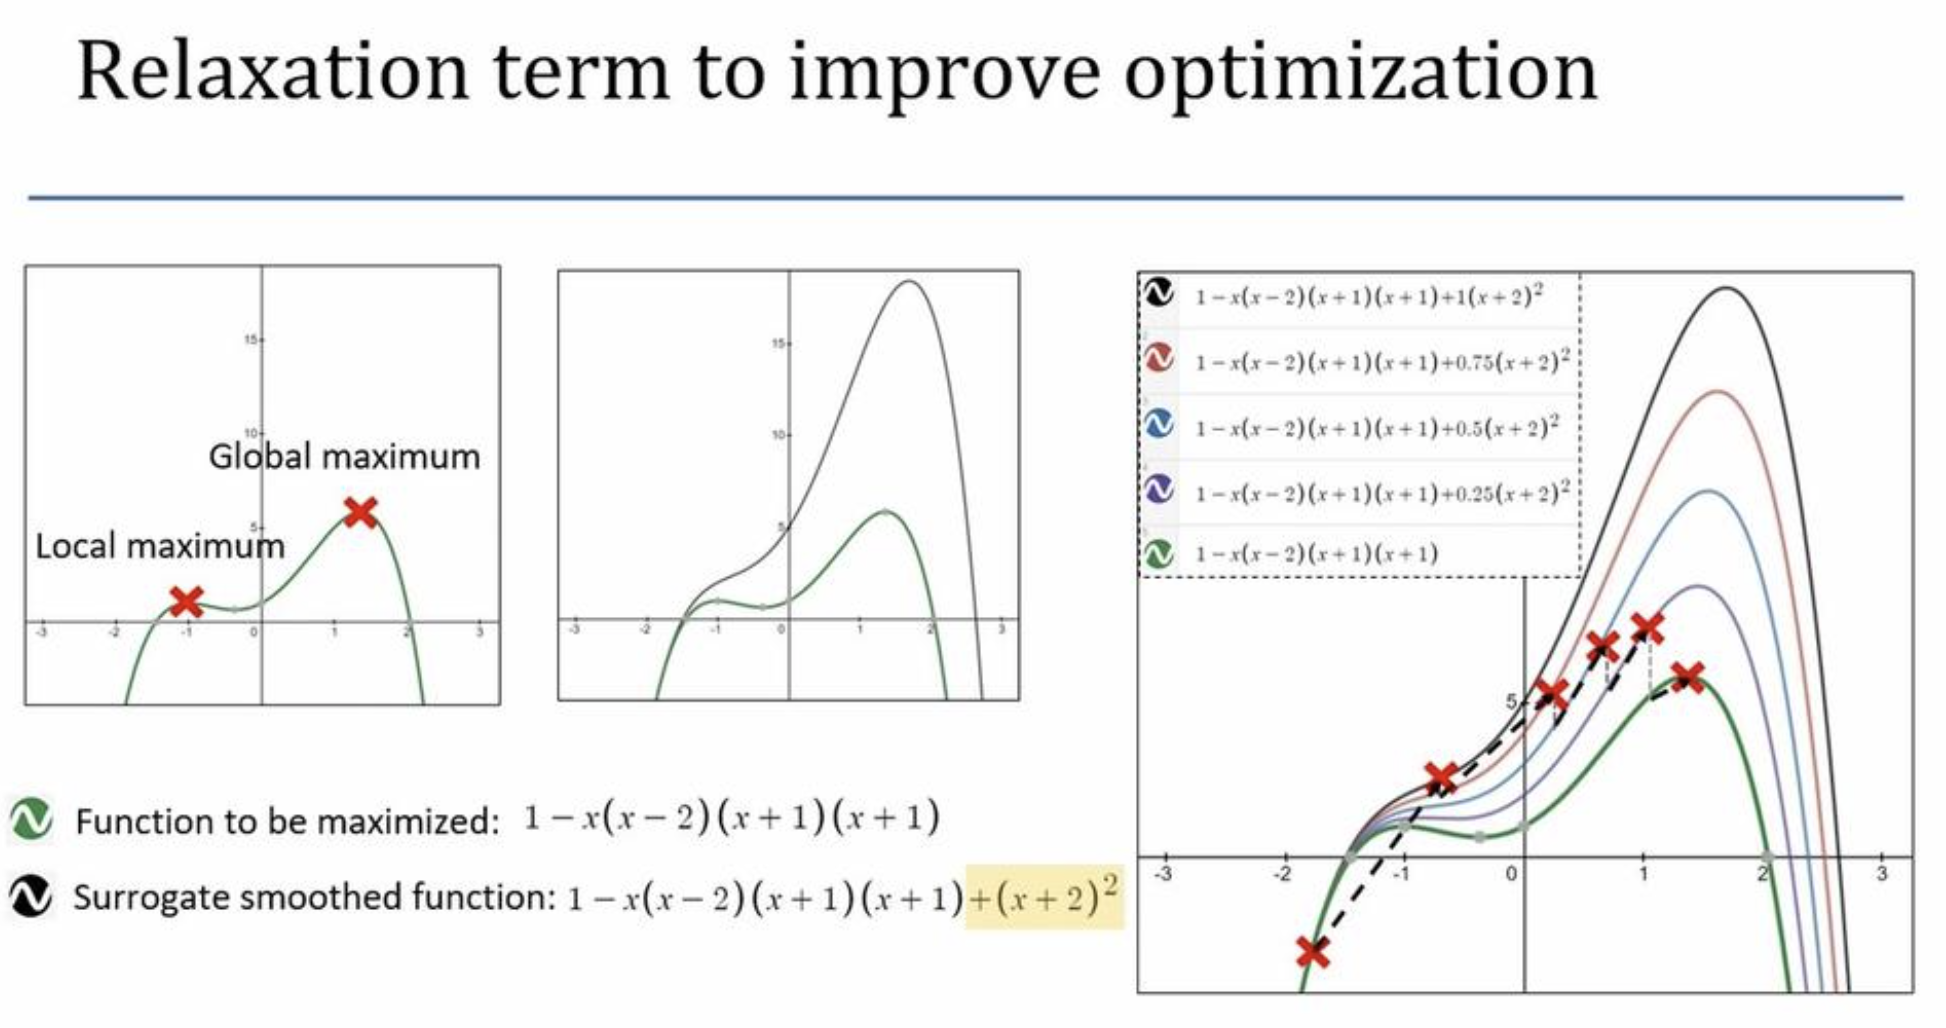
\includegraphics[scale=0.3]{neurips-2020/images/Screenshot 2020-12-10 at 21.11.50.png}
  \caption{1D example problem, which becomes more convex with introduction of the relaxation term. Loss surface becomes smoother hence leading to easier optimization and stronger attack.}
\end{figure}

{\bf Side note:} the requlization term is added with $\lambda$ parameter, which decays over optimization process and zeros-out at the end hence not effecting the ability of the system to reach an optimal solution. \\

{\bf Results:} stronger attacks with lower number of iterations (100 iterations are considered for almost all experiments in the paper). GAMA attack is tested not only against plain models, but also against current SOTA defences. \\

{\bf Key takeaways:} simple yet effective idea. The only disadvantage - only applicable for classification task, which limits its adoption in broader range of applications. \\









\subsection{Poster Session 4}
\subsubsection{Experimental design for MRI by greedy policy search \cite{BakkerHW20}}

Presented by \textit{Tim Bakker} \\

{\bf Motivation:} move away from handcrefted sampling masks towards learned aquisition strategies. \\

{\bf Observation:} the problem can be solved by joint optimization of some sampling scheme generator and the following reconstruction model. 
However, it leads to non-adaptive sampler: decision on which k-space lines to sample is made ones and not adjusted based on quality of recons made on partially sampled data. 
RL-based approach allows to make sampling scheme generation to be more adaptive. \\

{\bf Method:} an initial subsampling of k-space is obtained from the ground truth image.
The subsampled frequency domain is fed into a reconstruction method, which for neural network based reconstructions starts with an inverse Fourier transform. This intermediate step results in a zero-filled reconstruction.
The high-resolution reconstructed MR image is input to the policy network, which outputs a discrete probability distribution that represents the suggested sampling policy.
A action is sampled from this policy, corresponding to a measurement of k-space.
This measurement is simulated from the ground truth MR image, and the procedure is repeated until the acquisition budget is exhausted.
The reward of an acquisition step is given by the improvement in Structural Similarity Index of the ground truth and reconstruction resulting from that acquisition. \\

\begin{center}
  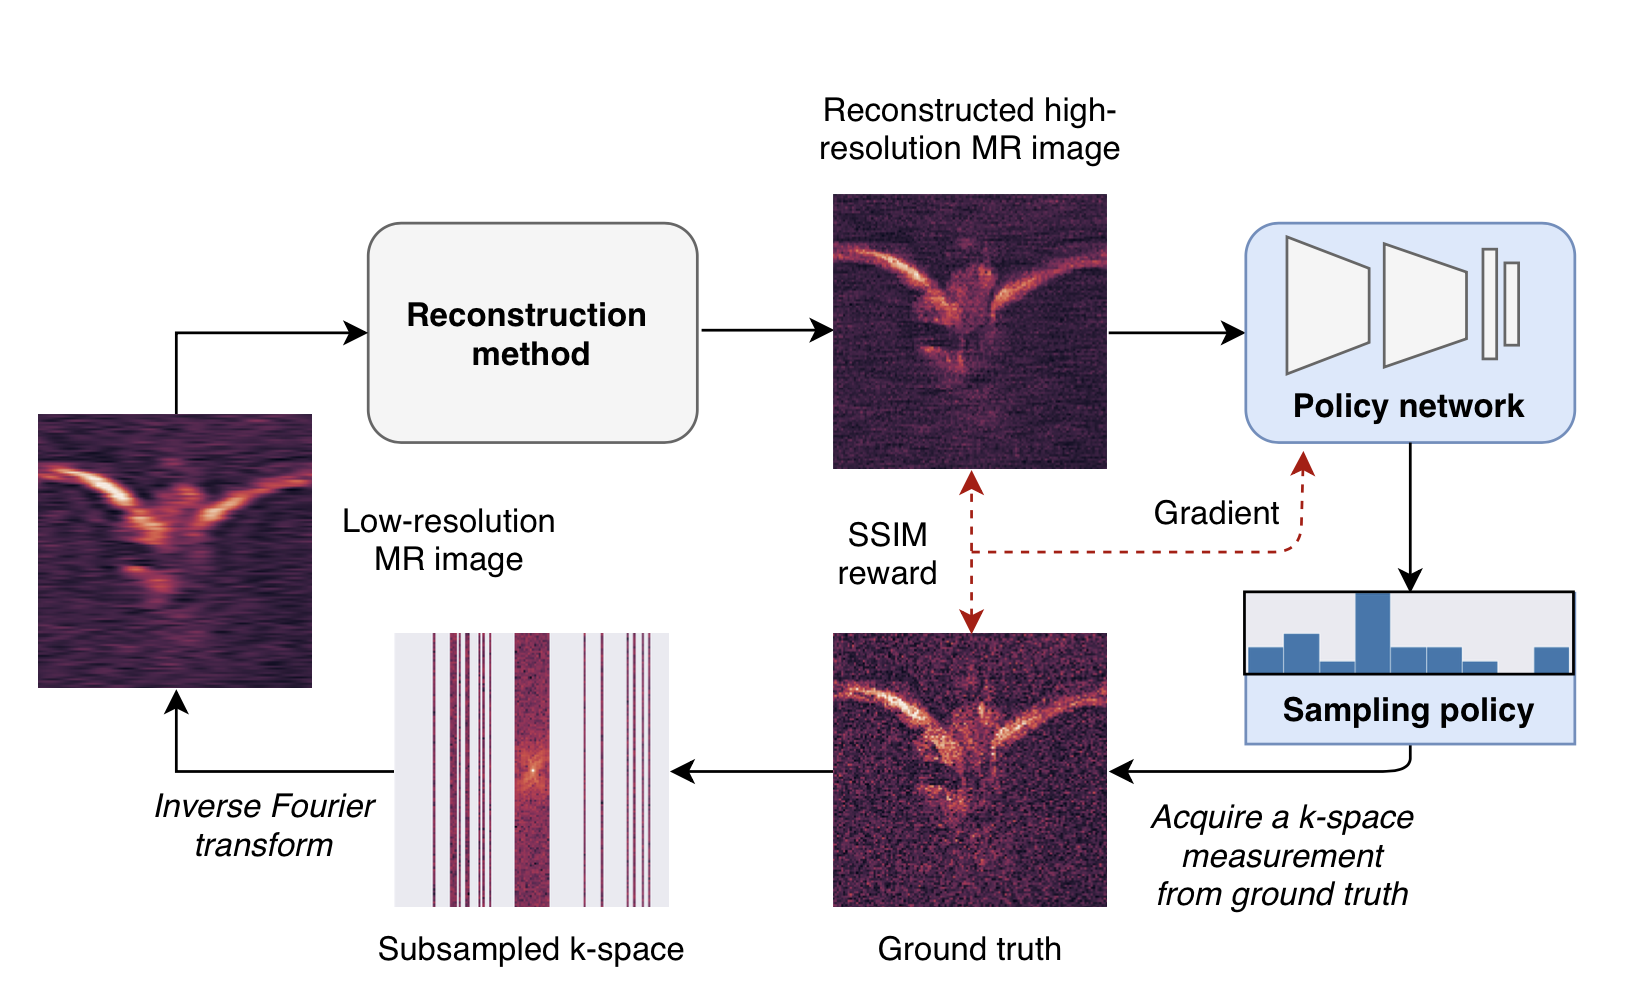
\includegraphics[scale=0.4]{neurips-2020/images/Screenshot 2020-12-10 at 11.12.09.png} \\
\end{center}

{\bf Side note:} of the biggest practical disadvantages of the approach is that reconstruction model is applied after each action $a$ meaning that several dozens of reconstruction may need to be performed before the desired resulting reconstruction is obtained. \\

{\bf Results:} results were only estimated base on SSIM values, no manual comparison with application specialists is done.
\begin{itemize}
    \item Based on SSIM values, Greed model performs better compared to other models. Learned policy was also compared with Random strategy that shares the initial mask with the other methods, and subsequently obtains a uniformly random measurement every acquisition step, similar to a simple VDS heuristic \cite{Lustig2007SparseMRI}
    \item The Greedy model is furthermore much less computationally expensive to train than any of the non-greedy models
    \item The Greedy model shows that it is adapting its predictions to individual MR images by outperforming the NA Oracle (selects as a measurement candidate in each acquisition step the column that leads to the greatest average SSIM improvement over the test dataset).
    This suggests that adaptivity is indeed a useful property for subsampling models to possess, and that this information can be learned in practice
    \item Method is verified for the single-coil case.
    It may be interesting to extend the work to more clinically relevant multi-coil case
\end{itemize} \\

{\bf Q\&A session with \textit{Tim Bakker}}

\textbf{Q:} How much is your learned policy better then some predefined one that people typically use?  
    
\textbf{A:} We have not made this comparison yet but there is a feeling that only application specialist will see the difference (remark: they do not have application specialists/clinical scientists in their research group) \\

\textbf{Q:} How much reconstructions from different policies are visually different?  

\textbf{A:} There is a huge gap in SSIM values but it is harder estimate visual difference (remark: seems like they have not done a proper visual evaluation) \\

\textbf{Q:} In the paper you tried to learn a policy with a fixed recon model. Have you consider a joint learning?  

\textbf{A:} We have not. However, we understand that joint optimization may lead to better results. It should be confirmed though (remark: our current SDF learning approach is joint and hence may be advantageous). \\

\textbf{Q:} Have you tried more clinically relevant (lower) acceleration factors?

\textbf{A:} Not really. We stick to the fastMRI accelerations of x4 and x8 and then proceeded with higher accelerations (x32) because we were interested what will happen with the agent and reconstructions. \\

\textbf{Q:} Have you considered non-cartesian sampling schemes?

\textbf{A:} Very little, it would be honest to answer no here. \\

\textbf{Q:} What are your plans? Are you going to develop the method further? (remark: the question was asked with an intent to find out about active sampling. However, I did not mention it explicitly) 

\textbf{A:} Not really. Currently, we are exploring options for clinical application and it draws all our attention. \\
